\subsection{Transitmethode}
\paragraph{Prinzip} Bedeckung des Sterns des Planeten\\
$\Rightarrow$ "`Einbruch"' in der Lichtkurve

\paragraph{Problem} Auswahleffekt $i$ im Bereich von $90\degree$
\paragraph{Vorteil} sehr kleine Planeten beobachtbar
\paragraph{Beispiel} HD209458 b
\begin{align*}
    i &= 87.1\degree & R_{\Pl} &= 1.27\,R_{\jupiter}
\end{align*}
\paragraph{RV-Messung} $M_{\Pl} \cdot \sin i = 0.63\, M_{\jupiter}$
\begin{align*}
    \Rightarrow M_\Pl &= \frac{0.63}{0.9987}\,M_{\jupiter} & M_{\jupiter} &= 1.197 \cdot 10^{30}\,\gram \\
    R_\Pl &= 1.27\,R_{\jupiter} = 9.067 \cdot 10^{7}\,\metre \\
    \Rightarrow \rho_\Pl &= \frac{M_\Pl}{\frac{4}{3} \pi R_\Pl^3} \approx 0.38\,\frac{\gram}{\metre^3} \tag*{$\rightarrow$ weniger dicht als Saturn}
\end{align*}

\paragraph{Satelliten-Missionen}
\begin{itemize}
    \item COROT
    \item Kepler
    \item PLATO (2024)
\end{itemize}

\subsection{Microlensing Methode}
\paragraph{Prinzip} Charakteristische Lichtkurve durch einen
Gravitationslinsenstern mit Planet

\paragraph{Situation}
\begin{center}
    \begin{minipage}[h]{0.5\textwidth}
        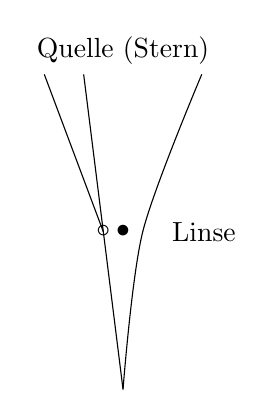
\begin{tikzpicture}
            \node (Quelle) at (0,4) {$\circledast$};
            \node [above] at (Quelle) {Quelle (Stern)};
            \node (Linse) at (0,2) {$\bullet$};
            \node [right,xshift=0.5cm] at (Linse) {Linse};
            \coordinate (Beob) at (0,0);

            \node at (-0.25,2) {$\circ$};
            \node at (1,4) {$\circledast$};
            \node at (-0.5,4) {$\circledast$};
            \node at (-1,4) {$\circledast$};

            \draw plot[smooth,tension=0.5] coordinates{(1,4) (0.25,2) (Beob)};
            \draw (-0.5, 4) -- (-0.25,2);
            \draw (-1, 4) -- (-0.25,2);
            \draw (-0.25,2) -- (0,0);
        \end{tikzpicture}
    \end{minipage}
    \begin{minipage}[h]{0.4\textwidth}
         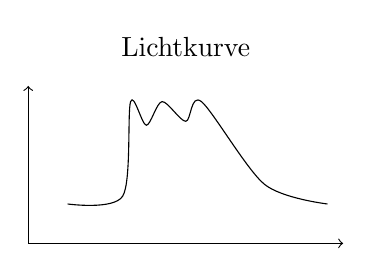
\begin{tikzpicture}
             \draw [->] (0,0) -- (4,0);
             \draw [->] (0,0) -- (0,2);
             \draw plot [smooth] coordinates{(0.5,0.5) (1.2,0.6) (1.3,1.8)
                                             (1.5,1.5) (1.7,1.8) (2,1.55)
                                             (2.2,1.8) (3,0.75) (3.8, 0.5)};
             \node at (2,2.5) {Lichtkurve};
         \end{tikzpicture}
    \end{minipage}
\end{center}

\subsubsection{Gravitationslinsen-Gleichung}
\paragraph{Annahme} Dünne Gravitationslinsen-Approxmation \\
$\Rightarrow$ lensing effect durch:
\begin{itemize}
    \item einzelne Materiensammlung
    \item in einer bestimmten Entfernung
\end{itemize}

\paragraph{Skizze}
\begin{center}
    \begin{tikzpicture}
        \coordinate (L) at (0,5);
        \node at (L) {$\bullet$};
        \node [anchor=south west] at (L) {$L$};
        \coordinate (S) at (3,7);
        \node at (S) {$\bullet$};
        \node [above] at (S) {$S$};
        \coordinate (S1) at (4.5,7);
        \node at (S1) {$\bullet$};
        \node [above] at (S1) {$S_1$};

        \draw [|-|] (-1.2,1) -- (-1.2,7) node [left,pos=0.5] {$D_S$};
        \draw [|-|] (-0.2,1) -- (-0.2,5) node [left,pos=0.5] {$D_L$};
        \draw [|-|] (-0.2,5) -- (-0.2,7) node [left,pos=0.5] {$D_{LS}$};

        \draw (60:0.5) -- (0,0) -- (120:0.5); 
        \draw (0,0) ++ (60:0.3) arc (60:120:0.3);
        \draw (0,1) -- (0,7);
        \draw (0,1) -- (S);
        \draw (0,1) -- (S1);
        \draw (0,7) -- (6,7) node [right] {Ebene der Quelle};
        \draw (L) -- (6,5) node [right] {Ebene der Linse};
        \draw (3,5) -- (S);
        \node at (1,5) [below] {$\xi$};
        \node at (1.5,7) [below] {$\eta$};
        \node at (3.75,7) [below] {$\varphi$};

        \draw (0,4.5) arc (270:360:0.5);
        \node at (0.2,4.8) {$\cdot$};
        \draw (2.5, 5) arc (180:90:0.5);
        \node at (2.8,5.2) {$\cdot$};
        \draw (3, 5) ++ (53.13:1.2) arc (53.13:90:1.2);
        \node at (3.3, 5.8) {$\tilde \alpha$};
        \draw [blue] (0,1) ++ (53.13:2) arc (53.13:90:2);
        \node at (0.5,2.5) {\color{blue} $\theta$};
        \draw [red] (0,1) ++ (63.43:3) arc (63.43:90:3);
        \node at (0.615, 3.4) {\color{red} $\beta$};
        \draw [green] (0,1) ++ (53.13:3) arc (53.13:63.43:3);
        \node at (1.4, 3.3) {\color{green} $\alpha$};
    \end{tikzpicture}
\end{center}

\begin{align*}
    \theta &= \beta + \alpha (\theta) \\
    D_S &= D_L + D_{LS}
\end{align*}o

\paragraph{Kleine Winkel}
\begin{align*}
    \beta &\approx \tan \beta = \frac{\eta}{D_S} \\
    \theta &\approx \tan \theta = \frac{\xi}{D_L} = \frac{\eta + \varphi}{D_S} > \beta + \alpha \\
    \alpha &\approx \frac{\varphi}{D_S} \Rightarrow \varphi = \alpha D_S = \tilde \alpha D_{LS}
\end{align*}

\paragraph{Annahme} local -- \textsc{Minkowski}-Raum (flach)
\[ \Rightarrow \boxed{\alpha = \left(\frac{D_{LS}}{D_S}\right) \tilde \alpha} \]

\begin{definition}
    \textbf{Ablenkungswinkel $\tilde \alpha$:} Lichtablenkung: Beschreibung durch
    "`Prismeneffekt"' \\
    $\hookrightarrow$ effektiven "`Brechungsindex"': $n = 1 + \frac{2}{c^2} \Phi$
\end{definition}

\paragraph{Gravitationspotential} $\Phi < 0$ 

\begin{align*}
    \tilde \alpha &= -\int \nabla_\bot n\ ds = -\int \nabla_\bot (1 + \frac{2}{c^2} \Phi)\ ds \\
                  &= -\frac{2}{c^2} \int \nabla_\bot \Phi\ ds
\end{align*}

\paragraph{Situation} Punktmasse $M$

\paragraph{Annahme} kleine Störung $\Rightarrow$ Integration entlang des ungestörten Weges \\
$b$: Impaktparameter

\begin{center}
    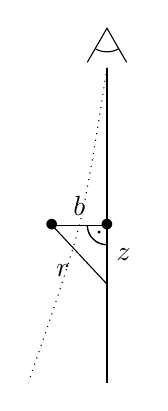
\begin{tikzpicture}
        \coordinate (S1) at (0,0);
        \coordinate (S) at (-1,0);
        \coordinate (M) at (-0.7,2);
        \node at (0,2) {$\bullet$};
        \node at (M) {$\bullet$};
        \draw [yshift=4.5cm] (240:0.5) -- (0,0) -- (300:0.5);
        \draw [yshift=4.5cm] (0,0) ++ (240:0.3) arc (240:300:0.3);
        \draw (S1) -- (0,4);
        \draw [dotted] plot[smooth,tension=0.5] coordinates{(0,4) (-0.7/2,2) (S)};
        \draw (M) -- (0,2) node [pos=0.5,above] {$b$};
        \draw (-0.25,2) arc (180:270:0.25);
        \node at (-0.1,1.9) {$\cdot$};
        \node [right] at (0,1.625) {$z$};
        \draw (M) -- (0,1.25) node [pos=0.5,anchor=north east] {$r$};
        \draw (-0.25,2) arc (180:270:0.25);
    \end{tikzpicture}
\end{center}

\paragraph{Bereich größter Annäherung}
\begin{align*}
    r &= \sqrt{b^2 + z^2} \\
    \Delta z &\approx \pm b \\
    \Phi(r) &= -\frac{GM}{r} = -\frac{GM}{\sqrt{b^2 + z^2}} = \Phi(b,z) \\
    \Rightarrow \nabla_\bot \Phi &= \frac{\partial}{\partial b} \Phi(b,z) \\
    \Rightarrow \tilde \alpha &= -\frac{2}{c^2} \int\limits_{-\infty}^{\infty} \frac{\partial}{\partial b} \left(-\frac{GM}{\sqrt{z^2 + b^2}}\right)\ dz \\
    &= \frac{2GM}{c^2} b \int\limits_{-\infty}^{\infty} \frac{1}{(b^2 + z^2)^{\frac{3}{2}}}\ dz
\end{align*}

Substitiution: $x := \dfrac{z}{b} \Rightarrow \dfrac{dx}{dz} = \dfrac{1}{b} \Rightarrow dz = b\ dx$

\begin{align*}
    \Rightarrow \tilde \alpha &= \frac{2GMb^2}{c^2} \underbrace{\int\limits_{-\infty}^{\infty} \frac{dx}{(1 + x^2)^{\frac{3}{2}}}}_{= 2} \cdot \left(\frac{1}{b^3}\right)\ dx \\
    &= \frac{2GM}{c^2b} \cdot 2 = \frac{4GM}{c^2 \cdot b} = \tilde \alpha
\end{align*}

\paragraph{Vergleich} Schwarzschildradius
\paragraph{"`Motivation"'} $v_{\mathrm{esc}} (R_S) = c$
\[ c = \sqrt{\frac{2GM}{R_S}} \Rightarrow \boxed{R_S = \frac{2GM}{c^2}} \]
$\Rightarrow$ \textbf{Ablenkwinkel:} $\boxed{\tilde \alpha = 2\left(\dfrac{R_S}{b}\right)}$

\paragraph{Beispiel} Ablenkung am Sonnenrand $\boxed{b = R_{\astrosun}}$
\[ \alpha = \frac{4GM_{\astrosun}}{c^2 R_{\astrosun}} = 1.7\arcsecond \]
\paragraph{Beobachtung} \textsc{Eddington} (1919): $20\,\%$ Bestätigung

\subsubsection{Einstein-Ring}
\paragraph{Bedingung} Quelle -- Linse -- Beobachter
\[ \beta{\Theta_E} = 0 \Rightarrow \underset{\mathclap{\text{Einstein-Radius}}}{\boxed{\Theta_E = \sqrt{\frac{D_{LS}}{D_S D_L} \frac{GM(\Theta_E)}{c^2}}}} \]
